\section{Análisis empírico}

\subsection{Performance para distribuciones uniforme}
A continuación mostraremos cómo se comportaron los distintos estimadores en cuanto al error medio obtenido ante la variación del parámetro $S$ (llamado $p$ en el código) de entrada del estimador en una distribución uniforme. Para cada $S$ fueron realizadas $100$ consultas por igualdad y $100$ consultas por mayor.

La distribución uniforme utilizada tiene 10000 elementos de 1 a 10000.


\begin{figure}[h!]  
  \centering
  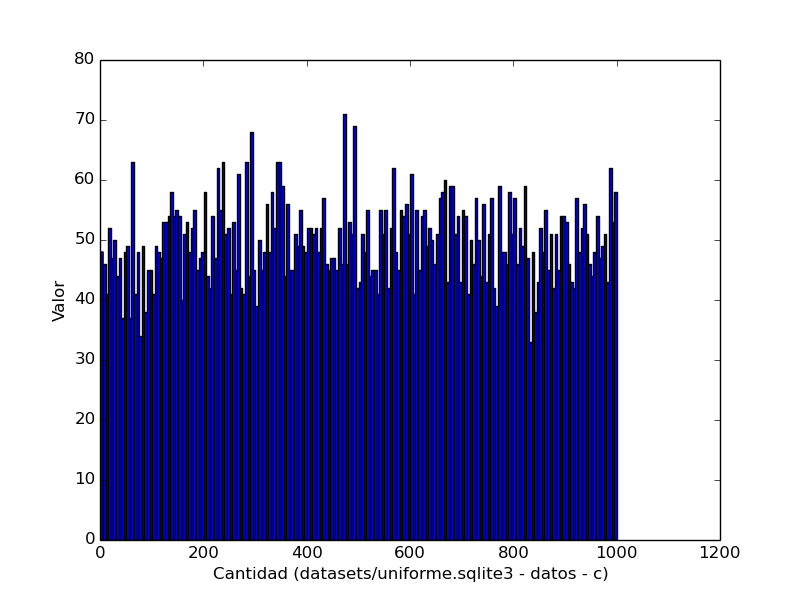
\includegraphics[width=0.45\textwidth]{../source/datasets/img/uniforme}
  \caption{Distribución utilizada}
 \end{figure}
 
\begin{figure}[h!]  
  \centering
  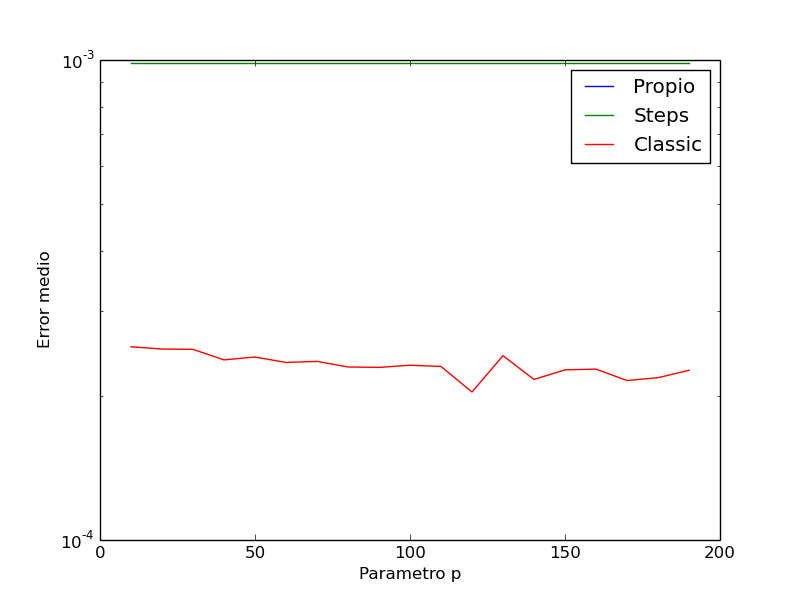
\includegraphics[width=0.45\textwidth]{../source/datasets/img/uniformeEqual}
  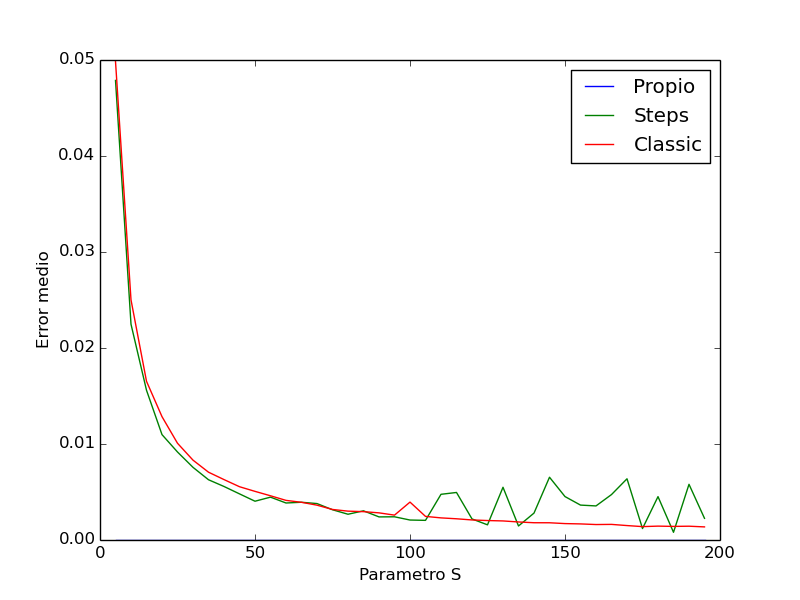
\includegraphics[width=0.45\textwidth]{../source/datasets/img/uniformeGreater}
  \caption{Error medio en función de $S$ para una distribución uniforme, con consultas por igualdad y por mayor respectivamente.}
 \end{figure}
 
 \subsubsection*{Análisis}
Estos datos confirman gran parte del análisis teórico que hicimos en la sección anterior. En primer lugar podemos ver cómo, en el caso de la estimación por igualdad, el parámetro del estimador no modifica de manera alguna la performance. Además, en ese caso la performance de ambos estimadores es muy buena (entre 0.0002 y 0.001), como también habíamos predicho. En el caso de la estimación por mayor confirmamos que en ambos estimadores, a diferencia de la estimación por igualdad, la elección del parámetro cambia drásticamente la performance obtenida, mejorándola al elevar el valor del parámetro.

Un resultado que no estaba contemplado en el análisis teórico es que a partir de cierto valor del parámetro la performance del estimador Distribution Steps oscila erráticamente. Creemos que esto se debe a que llega cierto punto en el que, al tener muchos buckets, comienza a haber valores que aparecen en más de un límite. En esa situación el algoritmo, como ya fue mencionado, caen en el caso en donde intenta minimizar el error en el caso peor caso, obteniendo una performance más pobre en el caso promedio. Intuitivamente podemos decir que pierde precisión al no poder ubicar unívocamente en qué bucket cae el $x_0$ de la consulta.
 
 \subsection{Performance para distribuciones normal}
A continuación mostraremos cómo se comportaron los distintos estimadores en cuanto al error medio obtenido ante la variación del parámetro $S$ de entrada del estimador en una distribución normal. Para cada $S$ fueron realizadas $100$ consultas por igualdad y $100$ consultas por mayor.

La distribución normal utilizada tiene 10000 elementos con $\mu=500$ y $\sigma=100$.


\begin{figure}[h!]  
  \centering
  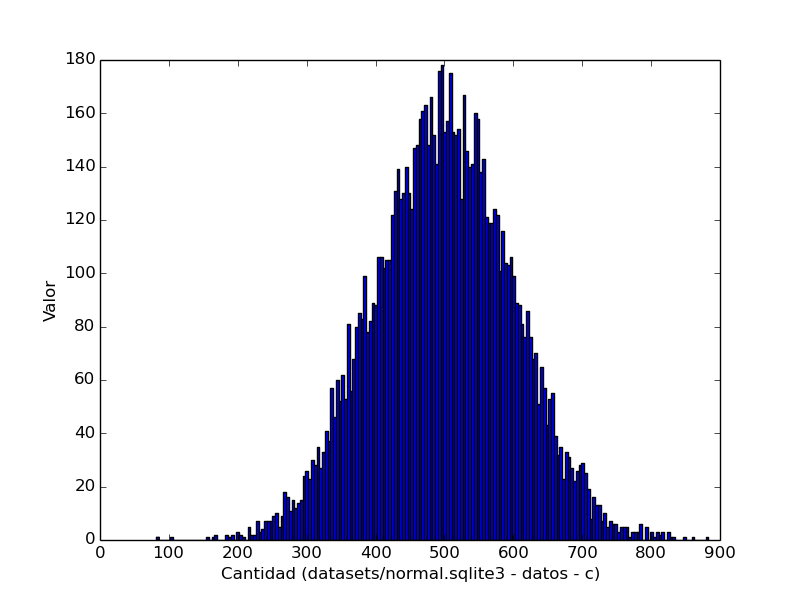
\includegraphics[width=0.45\textwidth]{../source/datasets/img/normal}
  \caption{Distribución utilizada}
 \end{figure}

\begin{figure}[h!]
  \centering
  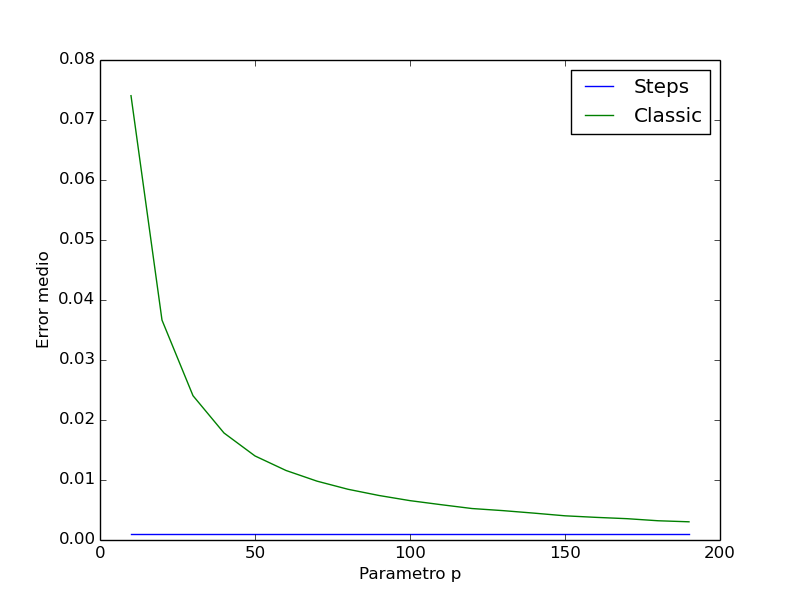
\includegraphics[width=0.45\textwidth]{../source/datasets/img/normalEqual}
  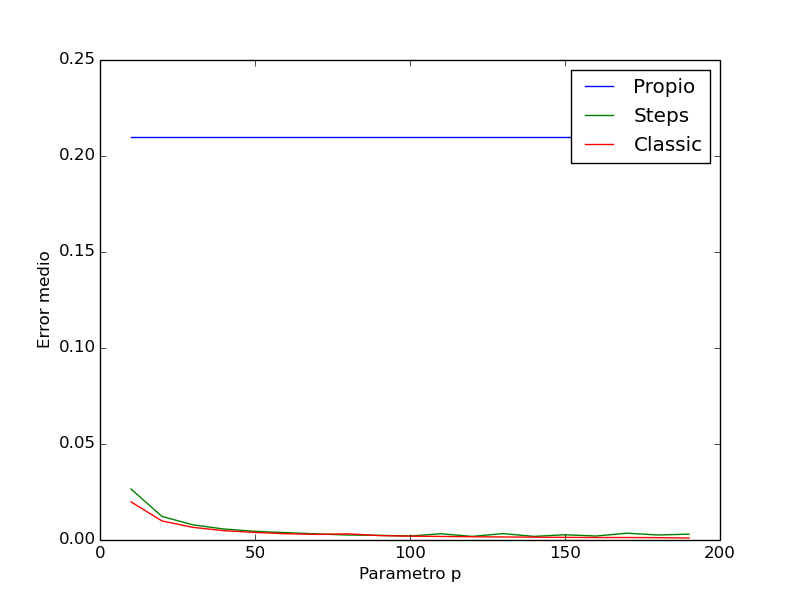
\includegraphics[width=0.45\textwidth]{../source/datasets/img/normalGreater}
  \caption{Error medio en función de $S$ para una distribución normal, con consultas por igualdad y por mayor respectivamente.}
 \end{figure}

 \subsubsection*{Análisis}
Gran parte del análisis es similar al caso uniforme con la excepción de que, como dijimos en el análisis teórico, el estimador clásico debería aumentar la performance al aumentar el parámetro. Esta mejora se aprecia únicamente en los primeros valores del experimento ya que llega rápidamente a una cantidad de buckets que le permite armar un histograma que caracteriza con precisión la distribución de este dataset. En este caso puede verse que el valor se encuentra alrededor de 10 pero en otros datasets este valor podría cambiar, e incluso necesitarse muchos más buckets para llegar al máximo nivel de performance, dependiendo mayormente del $\sigma$ de la distribución.

Observamos nuevamente el comportamiento errático de Distribution Steps para valores grandes de $S$, lo que aumenta la confianza en nuestra hipótesis de que el problema consiste en tener demasiada granularidad en los buckets.

\subsection{Performance para diferentes distribuciones}
En esta sección calculamos la performance de los estimadores en datasets de diferentes distribuciones provistas por la cátedra y análizamos, en cada caso, mediante un test de hipótesis, si alguno de los estimadores es significativamente mejor o si, en términos estadísticos, no existe una diferencia importante de performance. 
El test utilizado es el \textit{Student’s T-Test Apareado} y para realizarlo necesitamos tener dos conjuntos de datos emparentados que representen la información que queremos comparar. En nuestro caso, para comparar el estimador $A$ con el estimador $B$ en cierto dataset, calculamos por un lado la performance de $A$ para estimar valores individuales del dataset y, por otro lado, la performance de $B$ para estimar esos mismos valores. Esto nos da dos listas de datos que están emparentadas por los valores que se estan estimando. Los valores a estimar cubren todo el rango de valores del dataset en intervalos de 10 unidades. Era necesario calcular la performance individual para diferentes valores del dataset y no simplemente tomar la performance como el promedio de todos esos valores ya que el valor promedio no es suficiente información para llevar adelante un test de hipótesis de estas características.

Presentamos a continuación los gráficos de los datasets utilizados:

\begin{figure}[h!]
  \centering
  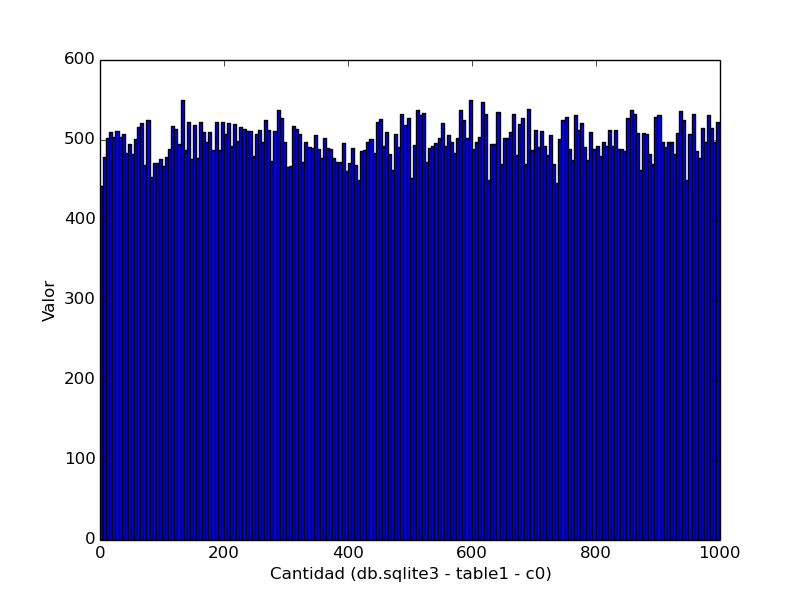
\includegraphics[width=0.45\textwidth]{./../source/datasets/img/c0}
  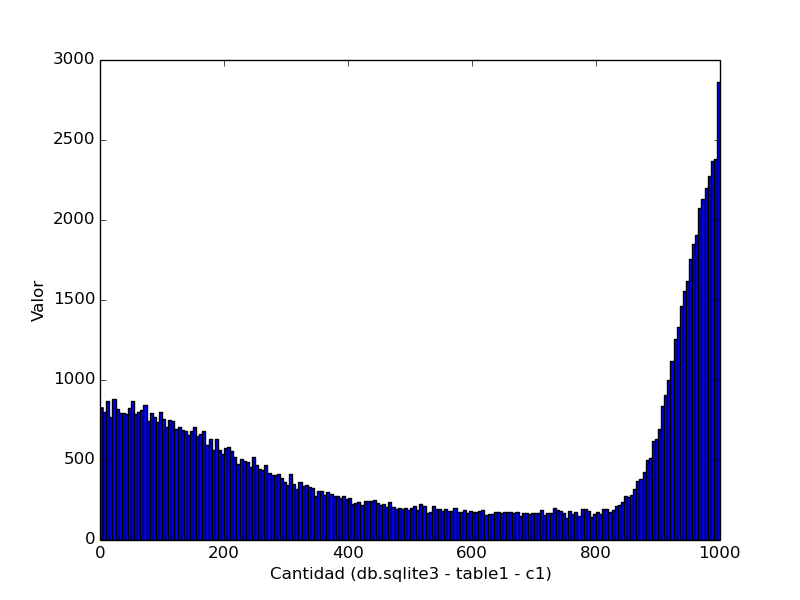
\includegraphics[width=0.45\textwidth]{./../source/datasets/img/c1}
  \caption{Gráficos de los datasets de las columnas c0 y c1}
 \end{figure}
 
 
\begin{figure}[h!]
  \centering
  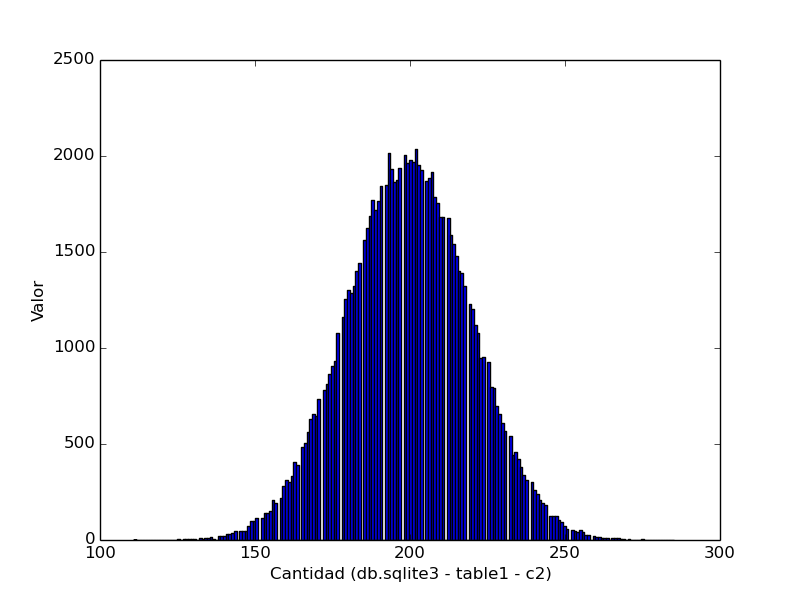
\includegraphics[width=0.45\textwidth]{./../source/datasets/img/c2}
  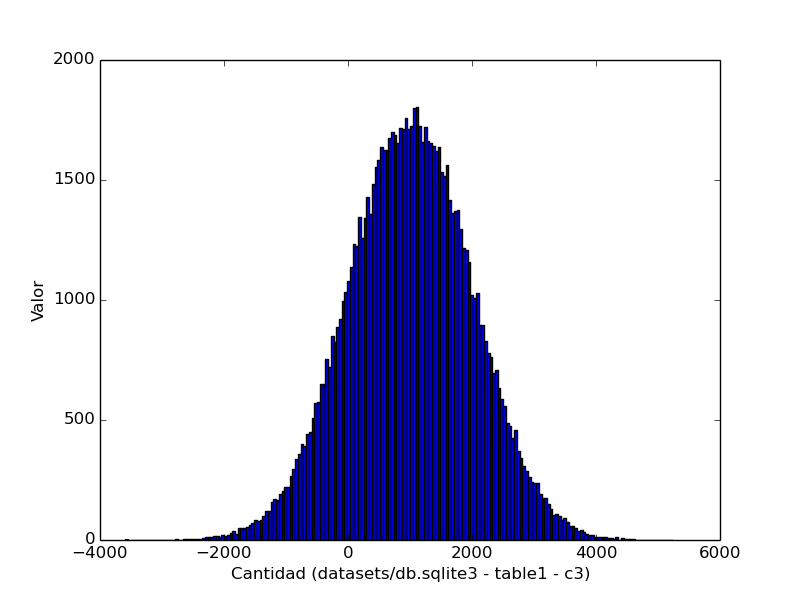
\includegraphics[width=0.45\textwidth]{./../source/datasets/img/c3}
  \caption{Gráficos de los datasets de las columnas c2 y c3}
 \end{figure}
 
\begin{figure}[h!]
  \centering
  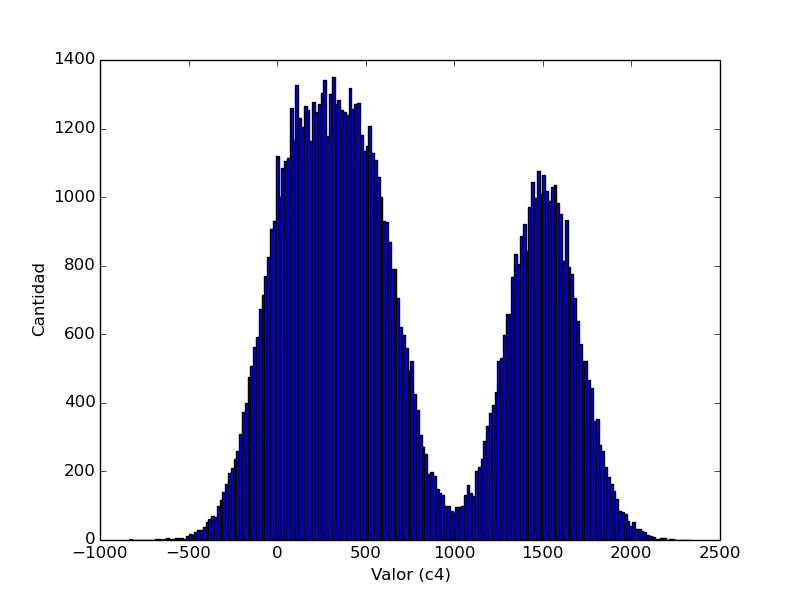
\includegraphics[width=0.45\textwidth]{./../source/datasets/img/c4}
  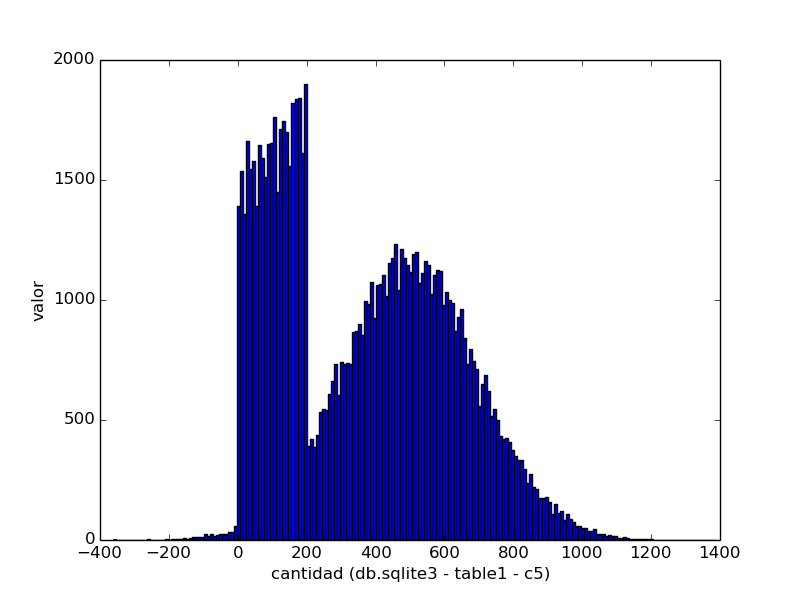
\includegraphics[width=0.45\textwidth]{./../source/datasets/img/c5}
  \caption{Gráficos de los datasets de las columnas c4 y c5}
 \end{figure}
 
 
\begin{figure}[h!]
  \centering
  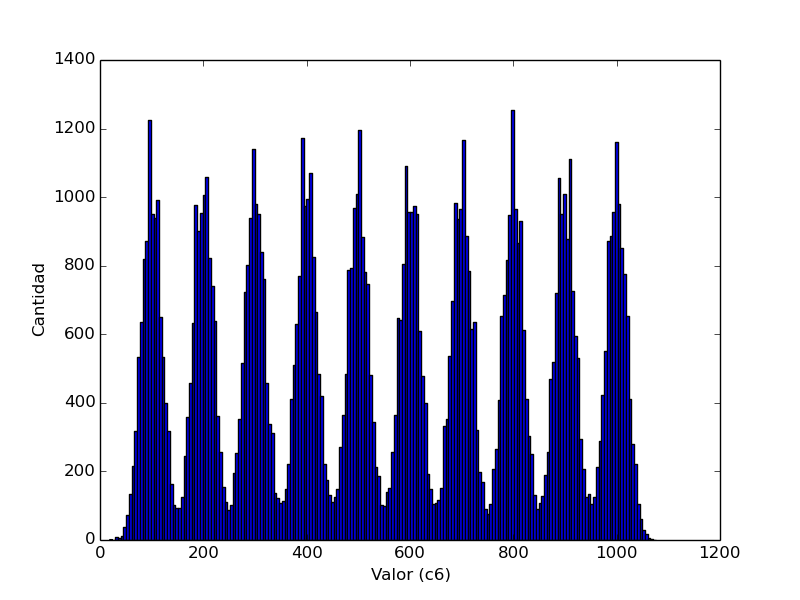
\includegraphics[width=0.45\textwidth]{./../source/datasets/img/c6}
  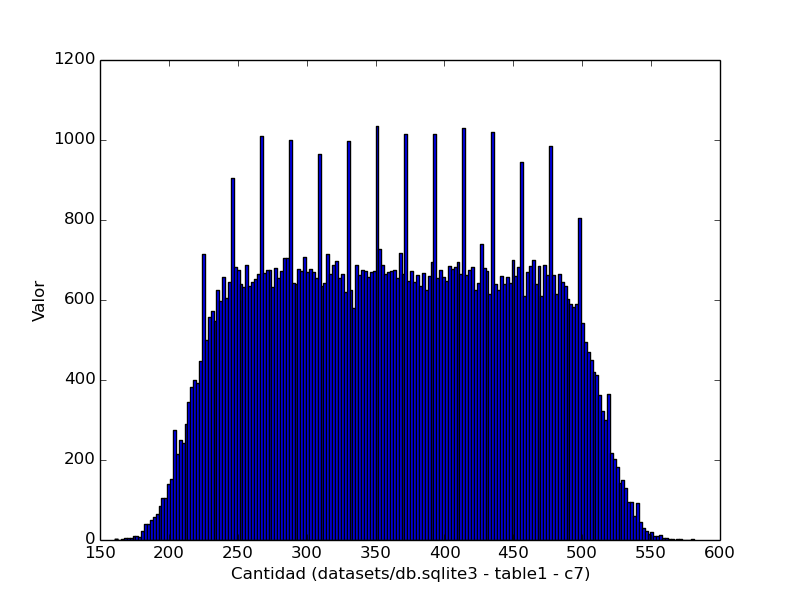
\includegraphics[width=0.45\textwidth]{./../source/datasets/img/c7}
  \caption{Gráficos de los datasets de las columnas c6 y c7}
 \end{figure}
 
 
\begin{figure}[h!]
  \centering
  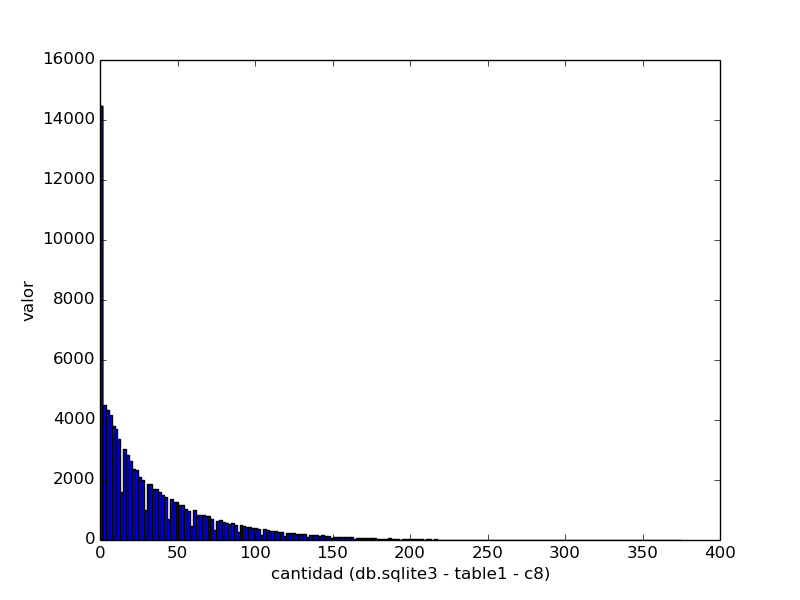
\includegraphics[width=0.45\textwidth]{./../source/datasets/img/c8}
  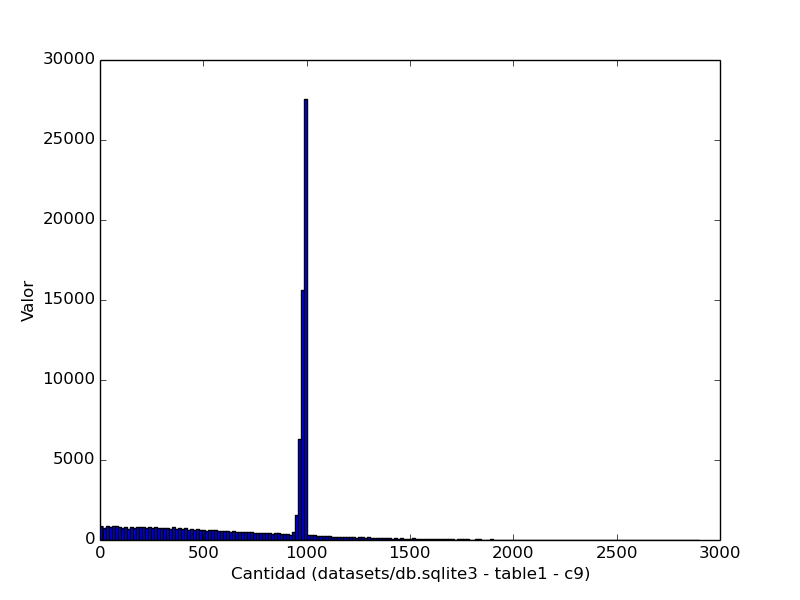
\includegraphics[width=0.45\textwidth]{./../source/datasets/img/c9}
  \caption{Gráficos de los datasets de las columnas c8 y c9}
 \end{figure}
 
\clearpage
Los estimadores que comparamos fueron los dos provistos por el paper y el nuestro, todos con $S=10$, en un enfrentamiento ``triangular''.
El cuadro indica, para una celda en la fila del estimador $X$, en la columna del estimador $Y$, subcolumna de selectividad $W$, en qué datasets de la tabla $X$ ``venció'' a $Y$ para la selectividad $W$, donde ``venció'' quiere decir que tuvo un menor error medio absoluto y que según el \textit{Student’s T-Test Apareado} la diferencia efectivamente fue significativa. La notación $i-j$ en una celda significa todos los valores entre $i$ e $j$, incluyendo ambos. Si un dataset $i$ no aparece ni en la celda $X, Y$ ni en la $Y, X$ para una misma selectividad $W$ hubo un ``empate'' (la diferencia no fue estadísticamente significativa) entre $X$ e $Y$ en ese dataset para esa selectividad.

\begin{table}[h!t]
\centering % centering table
\begin{tabular}{c rrrrrrr} % creating eight columns
\hline\hline %inserting double-line
\ &\multicolumn{2}{c}{Propio}& \multicolumn{2}{c}{Classic}& \multicolumn{2}{c}{Steps} \\ [0.5ex] 
\hline % inserts single-line
 & E & G & E & G & E & G &  \\  
\hline
Propio &X  &X  &0-7, 9 &0-9 &0-9 &0-9 \\ % Entering row contents
\hline
Classic &-  &-  &X &X &1-9 &6 \\
\hline
Steps &-  &- &- &0, 3-5 &X &X  \\[1ex] % [1ex] adds vertical space
\hline % inserts single-line
\end{tabular}
\caption{Comparación entre estimadores.} %title of the table
\label{tab:hresult}
\end{table}

\subsubsection*{Análisis}
Como se puede apreciar en el cuadro \ref{tab:hresult} podemos notar como el estimador creado por nosotros ``vence'' a los otros dos estimadores en todas las distribuciones. Esto se debe, como ya mencionamos, a su perfección a nivel de performance, aunque nuevamente vale recalcar que asume fuertemente que todos los elementos del dataset entran en memoria.
Es interesante analizar la comparación entre el estimador de Histograma Clásico y Steps en cada una de las distribuciones. Comencemos viendo las consultas por igualdad. En este caso el estimador Clásico es significativamente mejor en prácticamente todas las distribuciones. Esto se debe a que Distribution Steps resulta bastante malo para calcular igualdad, ya que como dijimos anteriormente en la sección 3 la densidad podría no aproximar bien la probabilidad de todo $x_0$. El único caso en que eso ocurre es en las distribuciones unifromes, y es precisamente allí donde Steps logra empatar con Classic. Podemos decir que para las consultas por igualdad Classic es claro vencedor.
Por otro lado, en las consultas por mayor, Classic ``vence'' a Steps sólo en el dataset 6 que presenta una distribución muy variable, creemos que esto es lo que perjudica la estimación de Steps. Pero Steps ``vence'' en los datasets 0, 3, 4, 5. En el 3, 4, y 5 puede deberse a que estas distribuciones presentan ciertos valores alrededor de los cuales se concentra la mayor parde de los datos, y en estos escenarios el Histograma Clásico corre el riesgo de meter gran porcentaje de los datos en un mismo bucket, con los problemas asociados que ya comentamos en repetidas ocasiones. Que Steps sea significativamente mejor en el caso del dataset 0 (una simple distribución uniforme) nos produjo cierto desconcierto, ya que no vemos la razón por la que pueda haber una diferencia significativa de performance. En este caso, de todos modos, el p-valor del test era 0.048 (muy cercano al umbral de 0.05 para considerarlo significativo), con lo puede tratarse simplemente de una ``anomalía'' estadística como las que mencionó Facu en la clase de presentación del TP.